\section{Evaluation}
\subsection{Evaluation Settings}

\subsubsection{Testbed}
For reproducibility and stability, we evaluated LODA over a server with 4 2080Ti 11GB GPUs, an Intel(R) Xeon(R) Silver 4116 2.10GHz CPU and 128 GB RAM.
When extending the number of robots involved, each robot is allocated a unique GPU to avoid performance bottleneck due to sharing GPU.


\subsubsection{Workload}
We choose a state-of-the-art implicit rendering method, BNV Fusion~\cite{li2022bnvfusion} as our workload, which reconstructs dense 3D mesh of the environment based on a sequence of depth images and their sampling poses.
BNV Fusion~\cite{li2022bnvfusion} is composed of a sparse grid of latent codes which is an implicit representation of the 3D environment and a pre-trained decoder.
% Given a depth image and its sampling pose, BNV Fusion predict a depth image corresponding to the sampling pose by decoding the latent codes using the decoder, compute mean square error between the predicted depth image and the input one as the loss and optimize the latent codes, forming an online training pipeline.
We use 2cm voxel size in BNV Fusion, other default hyper-parameters and the default decoder parameter checkpoint officially released.

% To support distributed training when the number of robots involved increases, we implemented ROG~\cite{guan_rog_2022} as the parameter synchronization backend which removes the parameter update synchronization barrier among the robots (robots do not need to synchronize parameter updates on every optimization step), enables partial parameter synchronization that has most contribution to performance of the AI model while ensuring convergence.
% The voxel size (proportional to the size of the local geometry for a local latent code) for the single 3D objects is 1cm to extract finer details and the voxel size for the Replica dataset is 2cm to save GPU memory and map a large scene.
% We also use the default hyper-parameters in its demo setting and use their released checkpoint for the encoder and the decoder.
% It is notable that the latent codes $\theta$ are only trained for 10 iterations on an NBV $v_{n+1}$ being input to $\bm{v_n}$ in BNV Fusion.


\subsubsection{Dataset}
We use the Habitat simulator~\cite{szot2021habitat} and Replica dataset~\cite{straub_replica_2019} commonly used in computer vision tasks. 
% The Habitat simulator renders high quality 3D scenes from the Replica dataset and simulates realistic physical trajectory of simulated agents in the 3D scene in real time and we ported it with the ROS stack by publishing its simulated output, including RGBD images and the poses of the simulated agents using the DDS of ROS.
We select three real-life high quality scenes from the Replica dataset of three levels of sizes: office\_0 sized 22.04$m^2$, hotel\_0 sized 35.88$m^2$ and frl\_apartment\_1 sized 93.10$m^2$, referred to as the small scene, the medium scene and the large scene.
The robots are spawned at random positions in the scenes.

The Habitat simulator broadcasts the simulated rgb samples of each robot at 10 Hz, and the online training task of BNV Fusion collects and processes the simulated output to optimize the training model at 1 Hz.
Every 2 minutes a reconstructed dense 3D mesh of the scene is produced to estimate the model's performance.


\subsubsection{Baselines}
We choose two state of the art active learning methods as our major baselines, namely Badge~\cite{ash_deep_2020} and ActiveNerf~\cite{avidan_activenerf_2022}.
Badge~\cite{ash_deep_2020} (referred to as badge) estimates the information gain of a possible input by computing the gradient magnitude and diversity with respect to parameters in the final (output) layer, which is computed using the most likely output according to the model.
% The diversity is measured by comparing the direction of the gradients with those of the existing input.
% And the one with highest magnitude and diversity is considered the most informative.
ActiveNerf~\cite{avidan_activenerf_2022} (referred to as uncertainty) is a method optimized for implicit rendering that models the training model output as a Gaussian distribution and add an extra model head that learns to predict the output variance as a measurement of uncertainty, where the zones with highest uncertainty is considered of highest information gain.
% They are both able to find the possible training input with highest information gain for the current training AI model, but would fail to provide a navigation path with highest accumulated information gain without considering the evolution of training AI model along the acquisition path.
To extend them to multiple robots, we duplicate these methods on each robot.
The baselines all use the same navigation stack as our system, with RRT* algorithm providing candidate training input for them to select from.


\subsubsection{Metrics}
To estimate the quality of the reconstructed mesh, we choose the completion ratio that is commonly used in 3D reconstruction tasks~\cite{li2022bnvfusion,zhu_nice-slam_2022}.
To calculate completion ratio, starting from vertices in the groundtruth mesh, we query for vertices in the reconstructed mesh whose distance is within a threshold and the ratio of successful query is the completion ratio, which reflects how close that the reconstructed mesh is to the groundtruth.
We also used Structure Similarity Index Measure (SSIM) to estimate the similarity between consecutive samples in breakdown to show how LODA instructs the robot to collect training input with higher diversity and quality.
SSIM close to 1 means that the two estimated images are identical, and SSIM smaller means less similar.


\subsection{End-to-End Performance}
\subsubsection{Different Sizes of Scenes}
\begin{figure*}[h!]
\centering
\vspace{-0.9cm}
\subfloat[office\_0 (Small Scene)]{
    \label{fig:single_small}
    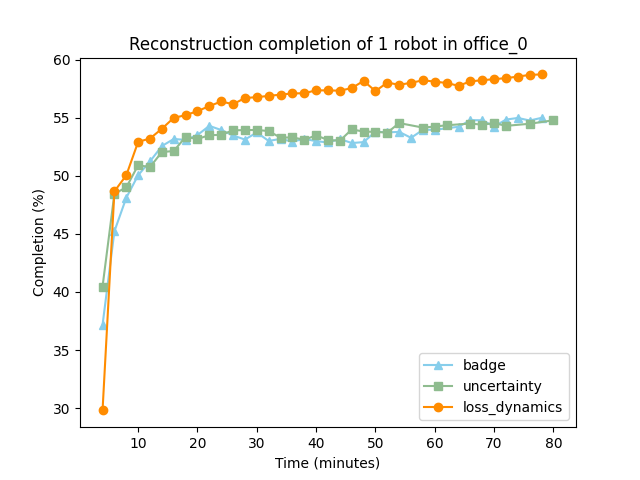
\includegraphics[scale=0.35]{fig/single/1_completions_plot_office_0.png}}   
\subfloat[hotel\_0 (Medium Scene)]{
    \label{fig:single_medium}
    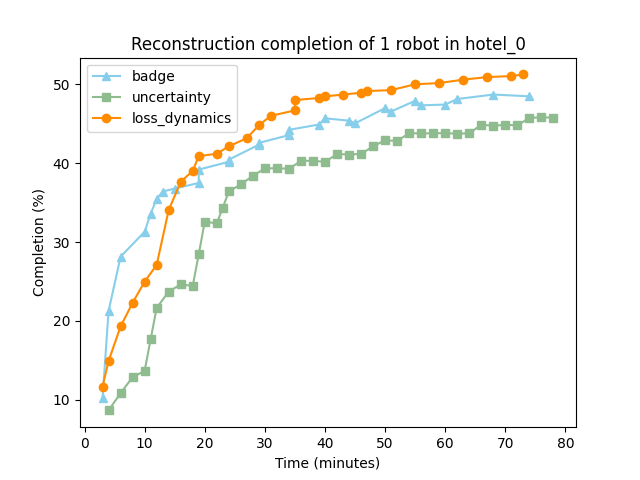
\includegraphics[scale=0.35]{fig/single/1_completions_plot_hotel_0.png}}
\subfloat[frl\_apartment\_1 (Large Scene)]{
    \label{fig:single_large}
    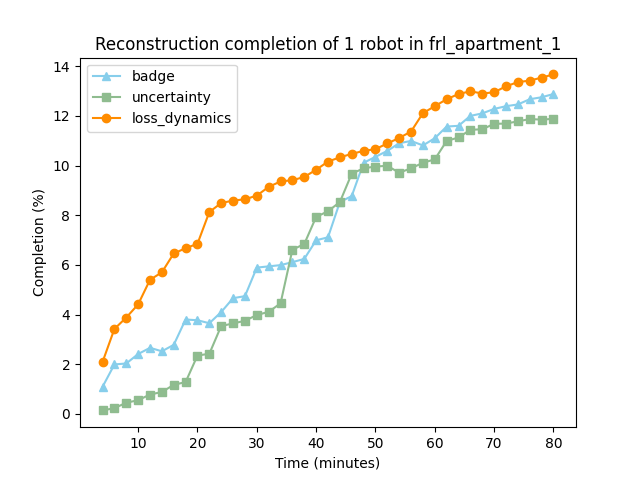
\includegraphics[scale=0.35]{fig/single/1_completions_plot_frl_apartment_1.png}}
\vspace{-0.3cm}
\caption{The completion ratio of the reconstructed mesh with one single robot in different sizes of scenes.}
\label{fig:single_robot}
\end{figure*}

We first compare the performance of three different methods (LODA referred to as loss\_dynamics in the figures) with one robot exploring and acquiring training data according to their information gain for the 3D reconstruction process in scenes of different sizes.
Note that the visible area of the whole scene to the four-wheel robot is limited because of the comparatively low perspective of a robot, the completion ratio in each scene is limited and lower than one hundred percent.

The experimental result in Fig~\ref{fig:single_robot} shows that our method outperforms the baselines across different scene sizes in terms of both time to reach the same completion ratio and the final completion ratio.
Compared with badge and uncertainty, LODA saved the time by about 43.8\% and 45.6\% for reconstruction completion ratio reaching 54\% in the office\_0 case,  by 21.5\% and 44.6\% for the completion ratio reaching 45\% in the hotel\_0 case and by 49.0\% and 49.8\% for the completion ratio reaching 8\% in the frl\_apartment\_1 scene
This can be attributed to LODA's ability to model the accumulated information gain of the whole navigation path and find the navigation path with highest accumulated information gain using the Loss Prediction Module and LODA-RRT algorithm.
% Figure \ref{fig:single_robot} illustrates the speeds at which one single robot, utilizing different active
% learning methods, reconstruct the mesh from the 3D scene with different sizes. 
% All three different sized scenes(small: Figure\ref{fig:single_small}, medium: Figure\ref{fig:single_medium}, and large: Figure\ref{fig:single_large}) prove that the advantage on reconstruction speed (xxx\% to xxx\%) of our method compared with two baselines remains, which can be attributed to the estimation of accumulated information gain along the whole candidate path with the LODA-RRT algorithm. 

Also, thanks to higher quality of training input sampled in LODA, the final completion ratio with LODA also increased across all the scenes.
Specifically, compared with badge and uncertainty, LODA achieved 4.1\% and 4.0\% higher completion ratio in the office\_0 case, 1.8\% and 6.7\% higher completion ratio in the hotel\_0 case and 1.1\% and 2.0\% higher completion ratio in the frl\_apartment\_0.

% Additionally, from Figure\ref{fig:single_small}, we can find that ours method achieve higher degree of completion (xxx\%) when our method and two baselines converge. 
% Such higher ceiling on completion degree shows that our method have the potential to reconstruct the mesh with higher quality compared with othger baselines.
% This is because baselines are viewing the training AI model in a static perspective. 
% As online training of the AI model proceeds, the parameters of the AI model keeps evolving and the possible training data of highest quality is also changed.
% In this way, baselines are unable to collect the training data of highest quality along the navigation path, leading to low quality of training data and lower quality of reconstruction.

\subsubsection{Different Numbers of Robots}

\begin{figure*}[h!]
    \centering
    \vspace{-0.8cm}
    \subfloat[office\_0 (Small Scene)]{
        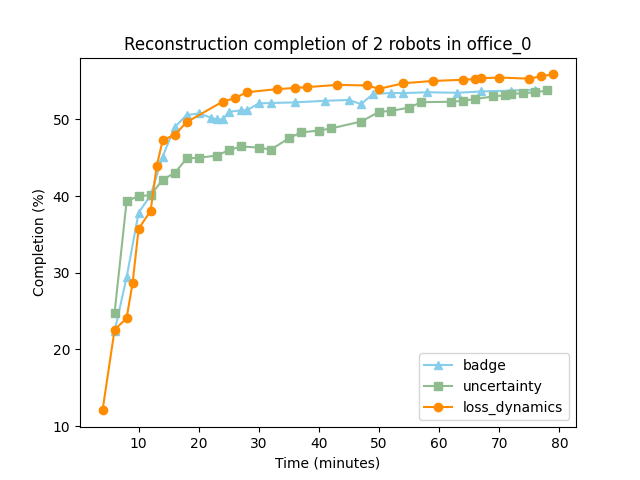
\includegraphics[scale=0.35]{fig/two/2_completions_plot_office_0.png}}   
    \subfloat[hotel\_0 (Medium Scene)]{
        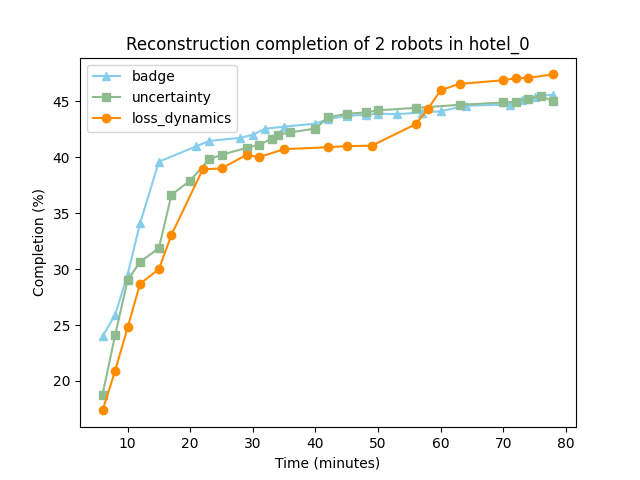
\includegraphics[scale=0.35]{fig/two/2_completions_plot_hotel_0.png}}
    \subfloat[frl\_apartment\_1 (Large Scene)]{
        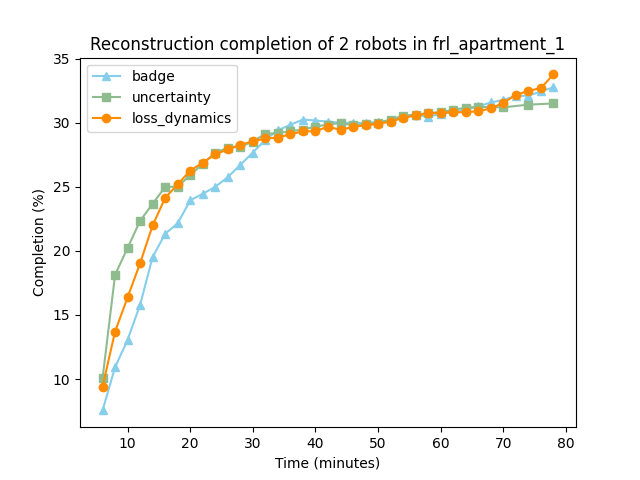
\includegraphics[scale=0.35]{fig/two/2_completions_plot_frl_apartment_1.png}}
    \vspace{-0.3cm}
    \caption{The completion ratio of the reconstructed mesh with two robots in different sizes of scenes. }
    \vspace{-0.1cm}
    \label{fig:two_robot}
\end{figure*}

We also carried out experiments of two robots exploring and taking training data in the same scenes.
And we found LODA still had the advantages of higher final reconstruction completion ratio:
compared with badge and uncertainty, LODA achieved 0.9\% and 1.0\% higher completion ratio in the office\_0 case, 1.7\% and 1.9\% higher completion ratio in the hotel\_0 case and 0.7\% and 2.5\% higher completion ratio in the frl\_apartment\_0.
But it can also be observed that the intensity of this advantages shrunk and the time to reach the same completion ratio was not evident.
This can be due to that while the baseline methods with a single robot tend to sample similar training input of low quality, duplicating them into multiple robots does extend their searching spaces for training data of high information gain and results in more diverse samples, mitigating their limitation and limiting LODA's advantages.
Nevertheless, the advantages in final completion ratio still reveal the contribution of the higher quality training data collected under the instruction of LODA.


% The experimental result shows that our method outperforms other baselines across different settings of robot number. 
% Figure X presents the training accuracy curves for different numbers of robots. 
% Under settings with 1, 2, and 3 robots, our method achieves higher accuracy than the baseline throughout the training process. 
% As the number of robots increases, the improvement in accuracy compared to the badge method further amplifies (from XX to XX). 
% This can be attributed to...  Additionally, at training times of XX, XX, and XX, our method exhibits a notable increase in accuracy growth, which can be attributed to ...

% figures: y accuracy; x time;
%  1 robot; 2 robots; 3 robots

%  fact

% ours all better than the baselines; more robot, diff larger
% badge, uncertainty > random, but due to ...
% with our system, ...

\subsection{Breakdown}

\begin{figure}[h!]
    \centering
    \vspace{-0.3cm}
    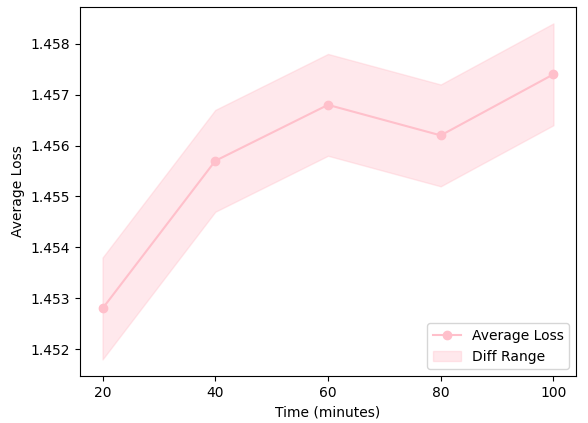
\includegraphics[width=0.7\linewidth]{fig/breakdown_prediction.png}
    \vspace{-0.3cm}
    \caption{Varying range of predicted loss and the actual loss.}
    \label{prediction}
    % \vspace{-0.5cm}
\end{figure}


In this section we inspect certain runtime statistics to better understand how LODA manages to acquire training data of higher quality.
First, we sampled and evaluated a test set sized 2000 for the Loss Prediction Module at each time spot indicated on Fig.~\ref*{prediction} in the one robot with office\_0 case and calculated the variation percentage $percent$ between the predicted loss $l_p$ and the groundtruth $l$ as $percent = \frac{\vert l_{p }- l \vert}{l}$.
The average of the variation percentage is recorded to be 1.84\% and the resulting variation range is depicted in Fig.~\ref{prediction}, which proves the effectiveness of the Loss Prediction Module.
% The average of the variation percentage is recorded to be 1.84\% and the resulting variation range is depicted in Fig.~\ref{prediction}, which proves the effectiveness of the Loss Prediction Module in modelling the loss dynamics and predicting future training loss based on rendered history of training loss from the Loss World Grid.
% This serves as a solid basis of the successive module of recursive path planning to estimate the accumulated information gain of paths and finding paths with optimal accumulated information gain.


\begin{figure}[h!]
    \centering
    \vspace{-0.3cm}
    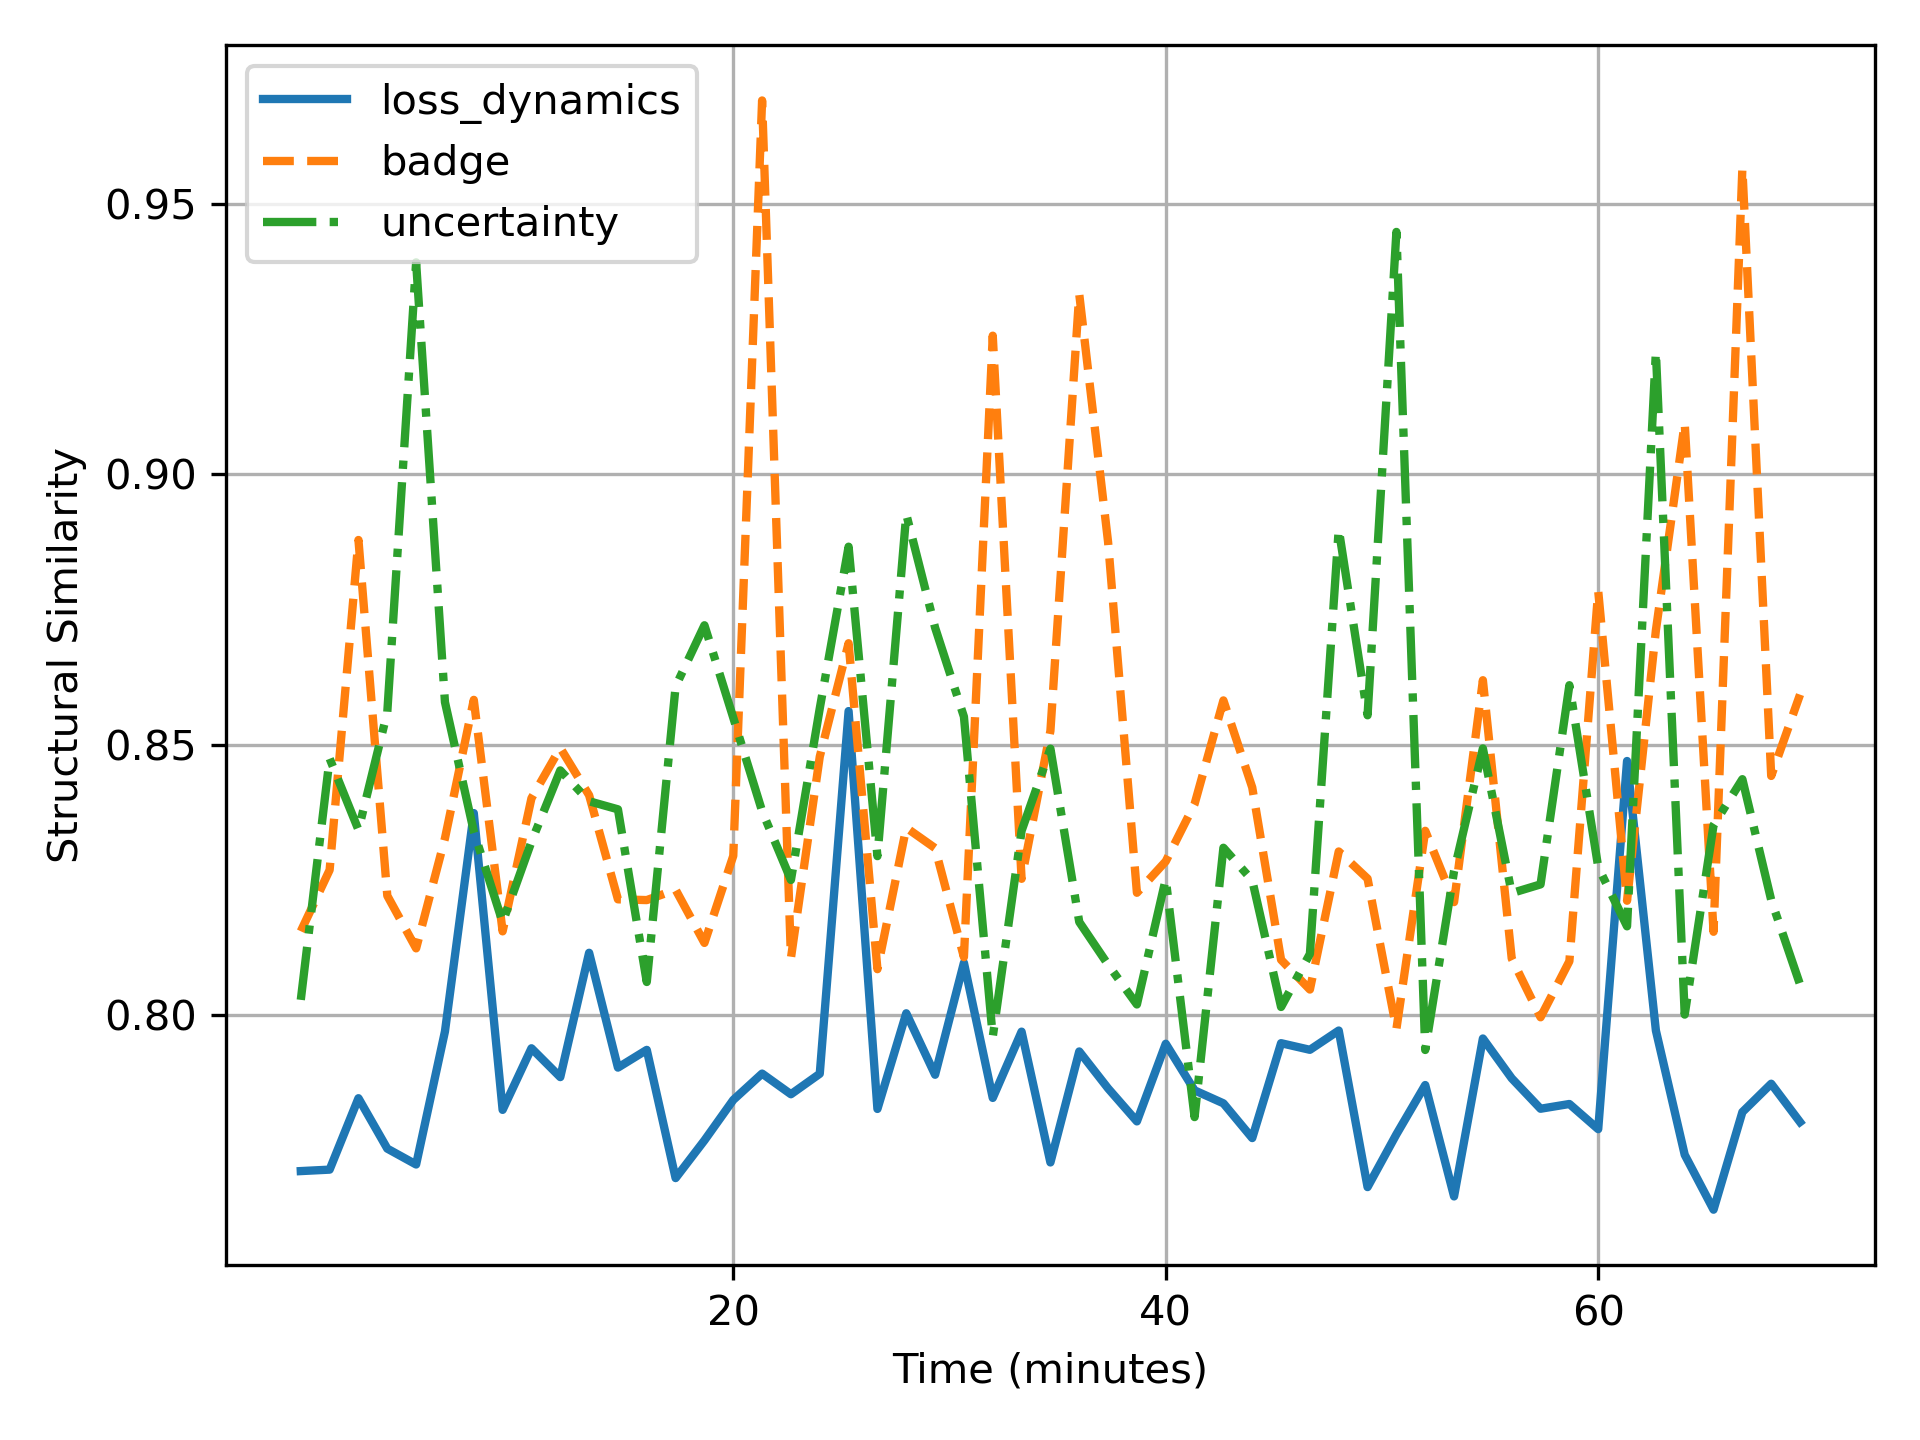
\includegraphics[width=0.7\linewidth]{fig/breakdown_similarity.png}
    \vspace{-0.5cm}
    \caption{SSIM between consecutive collected training data.}
    \label{similarity}
    \vspace{-0.7cm}
\end{figure}

\begin{table}[h!]
    \begin{center}
    \vspace{-0.3cm}
      \caption{Average SSIM between consecutively collected samples.}
    \vspace{-0.4cm}
      \begin{tabular}{c|c|c|c} % <-- Alignments: 1st column left, 2nd middle and 3rd right, with vertical lines in between
        \textbf{Methods} & loss\_dynamics & badge & uncertainty \\
        \hline
        \textbf{SSIM} & 0.789 & 0.843 & 0.840
        \label{table:similarity}
      \end{tabular}
    \end{center}
    \vspace{-0.3cm}
  \end{table}

Second, we calculated the SSIM values between depth images consecutively sampled across all evaluated methods in the  one robot with office\_0 case depicted in Fig.~\ref{similarity}, with average shown in Table.~\ref{table:similarity}.
We can learn that the baselines typically control the robot sampling depth images that are more similar than those collected under LODA.
% The recorded average SSIM is shown in Table.~\ref{table:similarity}.
Although lower SSIM does not directly translate into higher information gain between consecutive samples, higher SSIM does reveal the problem of the baselines that they tend to sample similar depth images when executing the planned path due to their static perspective of the training AI model.
% This also shows that LODA tends to control the robot to sample less similar samples under the instruction of the estimation of accumulated information gain along the candidate paths.




% \subsection{Discussion}